\pagestyle{empty}

\noindent \textbf{\Large A CD melléklet tartalma}

\vskip 1cm

\noindent A dolgozathoz tartozó melléklet a következőket tartalmazza.

\begin{itemize}
\item \texttt{dolgozat.pdf}: a dolgozat PDF fájl formájában,
\item \texttt{szakdolgozat}: a dolgozat \LaTeX\ forráskódját tartalmazó jegyzék,
\item \texttt{programok}: az elkészített programokat tartalmazó jegyzék.
\end{itemize}


A demók és program teszteléséhez szükséges egy kamera, egy marker (egy olyan, ami a megfelelő könyvtárba tartozik),
OpenCV, PyOpenGL,PyGame,ArUco, python3, falcon, waitress, requests és egyéb csomagok, amiket hiányolhat a futtatás közben.

Felhasználható marker: 
\begin{figure}[htp]
    \centering
   	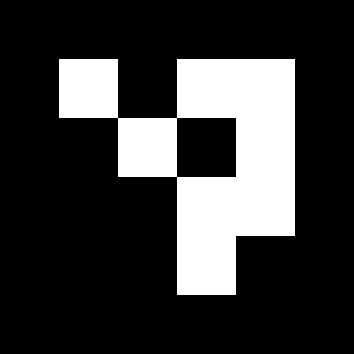
\includegraphics[scale=0.4]{images/marker.png}
	\caption{marker (forrás:https://chev.me/arucogen/)}
	\label{fig:marker}
\end{figure}

%Ami soknál felvolt használva forrás linkek :
%https://rdmilligan.wordpress.com/2015/10/15/augmented-reality-using-opencv-opengl-and-blender/
%http://openglsamples.sourceforge.net/cube_py.html 
%https://stackoverflow.com/questions/50764623/object-is-wrong-displaced-in-ar-aruco-opengl
%https://realpython.com/python-timer/
%https://www.pygame.org/wiki/OBJFileLoader
%képekről link modellekről link? :)


\begin{itemize}
\item \textbf{program} (a végső program): 
\begin{itemize}
\item \textbf{Játékleírás}: A játék célja a dobozok eltüntetése, a szökőkutakba kell bele tolni őket.
Minden pingvin csak a saját színével megegyező dobozt tolhatja, egyszerre csak egy kút aktív és
pontosan annyi doboz kell bele amennyi játékos van. Ha megfelelő számú doboz kerül bele, az eddig nem aktív kút lesz az aktív.
Ha minden doboz eltűnik, akkor ér véget a játék,nyernek a játékosok.  
Minden játékoshoz 4 doboz tartozik, maximum négy fő vehet részt a játékban.
\begin{figure}[htp]
    \centering
   	
\includegraphics[scale=0.1]{images/win.jpg}
	\caption{A játék vége(forrás:https://miro.medium.com/max/500/1\*KOj47lkJHi9w8bxAvFAvEg.jpeg)}
	\label{fig:win}
\end{figure}
\item \textbf{Tesztelési lehetőség}: el kell indítani a server.py-t, aztán pedig a game.py-t, ez egyetlen kliens-t szimulál.
Ha nem állítódik le a server.py, de a game.py újraindítódik, akkor az már a következő kliensek számít.
A játék jelenleg 2 klienssel működik, de ezt lehet bővíteni a kezdőadatok megadásával.
\end{itemize}
\item \textbf{demos}:
\begin{itemize}
\item aruco\_test:
A \textbf{test\_aruco.py} fájlt kell futattni.
Az ArUco maker detektálására készítette program kód teszje. 

Az images mappában szerepel 12 kép, azokon próbálja felismerni a markert, ha sikerül kirajzolja a közzépponthoz
tartozó triédert és visszaadja a marker eltolását és elforgatását kamerához képest. (rvec, tvec)
Az eredmény ( a kép és az adatok) a result mappába kerülnek.
\item camera\_background\_with\_obj :
A \textbf{camera\_cap\_with\_obj.py} fájlt kell futattni.
A kamera képből textúra készül, majd beállítódik háttérnek és kirajzolódik rá egy objektum.

Az obj objektum és mtl textúra betöltése az objloader.py-jal történik.
A pingin modell a models mappában található.
Kilépés 'q'-val történik.
\item camera\_calibration :
A \textbf{calibration.py} fájlt kell futattni.
A kamera kalibrációja OpenCV és sakktábla minta használatával.
A kalibrációhoz felhasznált képek az Images mappában találhatók.

Az eredmény a log.json-ben tárolódik.
Ebbe az álományba mentődik ki a kamera mátrix és a disztorziós együtthatók.

A harmadik fejezetben említett kalibrációs kód a megjelölt forrásban szereplő kódot használtam fel hozzá. 
%https://medium.com/@aliyasineser/opencv-camera-calibration-e9a48bdd1844
\item camera\_calibration\_and\_aruco\_demo:
A \textbf{calibration.py} fájlt kell futattni.
A harmadik fejezetben említett demó, a megjelölt forrásban szereplő kódot használtam fel hozzá. 
%https://medium.com/@aliyasineser/aruco-marker-tracking-with-opencv-8cb844c26628
\item camera\_func:
A \textbf{camera.py} fájlt kell futattni.
Az aktuális kameraképet visszaadó funkció szerepel benne. 
\item camera\_texture\_on\_a\_cube:
A \textbf{cam\_cap\_texture\_on\_cube.py} fájlt kell futattni.
A kamera képből készült textúra kerül egy kirajzolt kockára.
\item draw\_cube:
A \textbf{draw\_cube.py} fájlt kell futattni.
Egy színes oldalapokkal rendelkező kocka rajzolódik ki egy GLUT ablakba.
\item draw\_scene:
A \textbf{draw\_scene.py} fájlt kell futattni.
A játék egy lehetséges kezdő állását bemutató rövid programkód.
(Végül nem így néz ki.)
\item draw\_texture\_from\_camera:
A \textbf{camera\_cap\_texture.py} fájlt kell futattni.:
Az aktuális pillanatnyi kamera képből textúra készül és ez a 
textúra a beállítódik egy GLUT ablak háttereként. 
\item draw\_trieder:
A \textbf{draw\_trieder.py} fájlt kell futattni.
A (0,0,0) pontba kirajzolódik egy triéder.
\item game:
A \textbf{game.py} fájlt kell futattni.
\item game\_with\_aruco:
A \textbf{game.py} fájlt kell futattni.
%https://realpython.com/python-timer/
\item keyboard:
A \textbf{keyboard.py} fájlt kell futattni.
A (0,0,0) pontba kirajzolódik egy triéder. A nyíl billyentyűkkel előre, hátra illeve 
két oldalra lehet mozogni.
A space megnyomása után felfelé mozdul el a kamera.
\item keyboard\_with\_cube:
A \textbf{keyboard\_cube.py} fájlt kell futattni.
A (0,0,0) pontba kirajzolódik egy triéder és egy kocka. A nyíl billyentyűkkel előre, hátra illeve két oldalra lehet mozogni.
A space megnyomása után felfelé mozdul el a kocka.
\item keyboard\_with\_obj:
A \textbf{keyboard\_obj.py} fájlt kell futattni.
A (0,0,0) pontba kirajzolódik egy triéder és betöltödik a pingvin modell.

A nyíl billyentyűkkel előre, hátra illeve  két oldalra lehet mozogni.
A space megnyomása után felfelé mozdul el.
\item load\_grab\_animation:
A \textbf{grab.py} fájlt kell futattni.
Betöltődnek a models mappában található pingvin modellek és kirajzolódnak váltva egymást a mozulatok
világos kék háttére. Van a mozdulatok között egy kis késeltetés.
Az animáció a doboz tolásához a kéz emelése.
\item load\_jump\_animation:
A \textbf{jump.py} fájlt kell futattni.
Betöltődnek a models mappában található pingvin modellek és kirajzolódnak váltva egymást a mozulatok
világos kék háttére. Van a mozdulatok között egy kis késeltetés. 
Az animáció az ugrás.
\item load\_obj:
A \textbf{load\_obj.py} fájlt kell futattni.
Betöltődik a models mappában található pingvin modell és kirajzolódik egy
világos kék háttére.
\item load\_release\_animation:
A \textbf{release.py} fájlt kell futattni.
Betöltődnek a models mappában található pingvin modellek és kirajzolódnak váltva egymást a mozulatok
világos kék háttére.

Van a mozdulatok között egy kis késeltetés.
Az animáció a doboz tolása utána a doboz elengedése.
\item load\_walk\_animation:
A \textbf{walk.py} fájlt kell futattni.
Betöltődnek a models mappában található pingvin modellek és kirajzolódnak váltva egymást a mozulatok
világos kék háttére. Van a mozdulatok között egy kis késeltetés. 
Az animáció a sétálás.
\item makeGlutWindow:
A \textbf{glutwindow.py} fájlt kell futattni.
Üres GLUT ablak nyitása, glutMainLoop használata.
\item simple\_camera:
A \textbf{camera.py} fájlt kell futattni.
A kamera kép lekérése és megjelenítése OpenCV segítségével.
Kilépés 'q'-val történik.
\item trackAruco:
A \textbf{trackAruco.py} fájlt kell futattni.
A kamera kalibrációja során megkapott mátrixot és együtthatókat betöltve és
felhasználva marker detektálás egy kapott képen.
Ha talál markert vissza adja a marker eltolását és elforgatását kamerához képest. (rvec, tvec)
\item trackAruco\_and\_draw\_Castle:
A \textbf{track\_and\_draw.py} fájlt kell futattni.
Aruco marker felismerés majd egy kastély modell rajzolása a markerre.
\item trackAruco\_and\_draw\_Cube:
A \textbf{track\_and\_draw.py} fájlt kell futattni.
Aruco marker felismerés majd egy kocka rajzolása a markerre.
\item trackAruco\_and\_draw\_model:
A \textbf{track\_and\_draw.py} fájlt kell futattni.
Aruco marker felismerés majd egy pingvin modell rajzolása a markerre.
\end{itemize}
\end{itemize}